\section{Pregunta N$^{\circ}$12\qquad Carlos Alonso Aznarán Laos}

\begin{frame}
    \begin{enumerate}\setcounter{enumi}{11}
        \item

              Sea
              \begin{math}
                  f\left(t\right)=
                  \dfrac{1}{1+t^{2}}
              \end{math}
              para $t\in\left[-5,5\right]$, utilizando un polinomio
              interpole $f$ en $n$ puntos igualmente espaciados de
              $\left[-5,5\right]$.
              Considere $n=5,8,10$ y compare con $f$ usando una
              gráfica.
    \end{enumerate}

    \begin{solution}
        \begin{figure}[ht!]
            \centering
            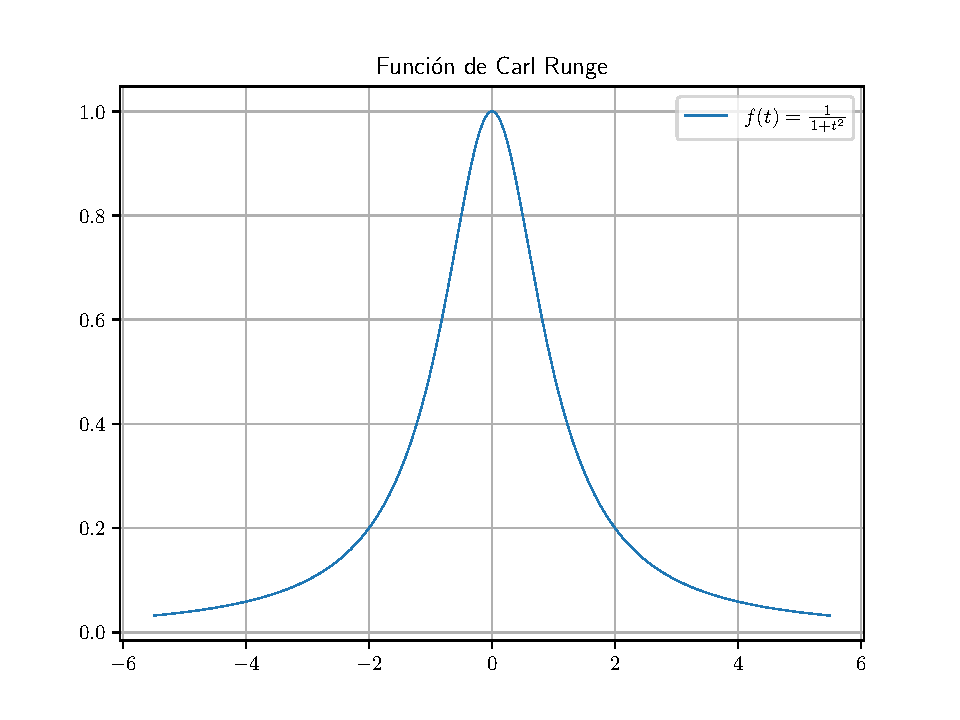
\includegraphics[width=.72\paperwidth]{p12}
        \end{figure}
    \end{solution}
\end{frame}

\begin{frame}
    \begin{solution}
        \begin{equation*}
            P_{4}\left(t\right)=
            0.005305t^{4}-
            0.1711t^{2}+
            5.79\times 10^{-17}t+
            1.
        \end{equation*}
        \begin{figure}[ht!]
            \centering
            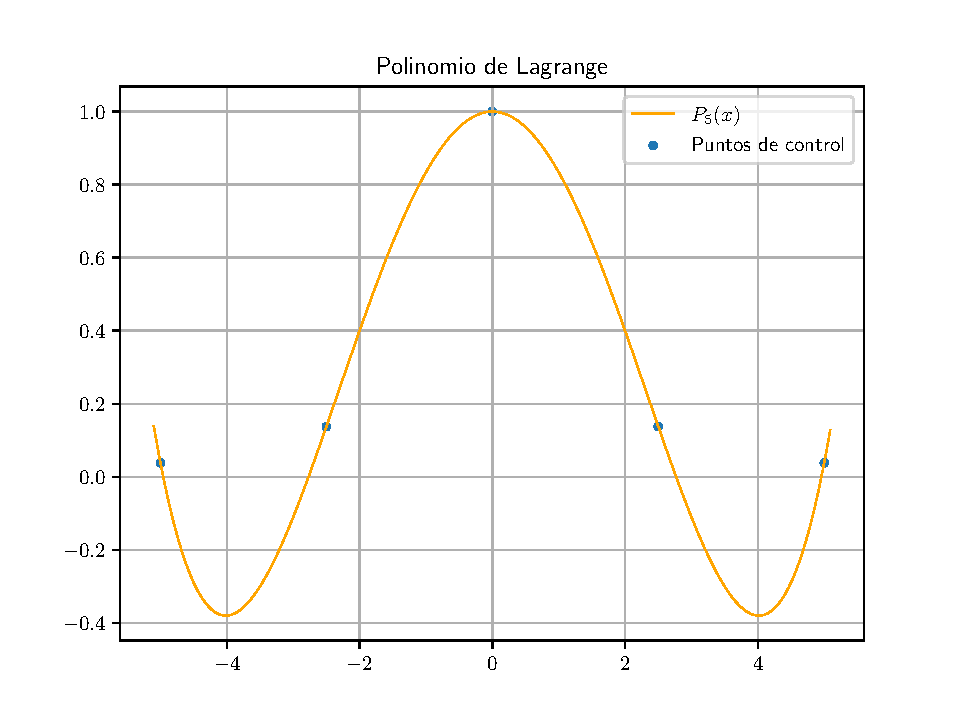
\includegraphics[width=.5\paperwidth]{p12_lagrange5}
        \end{figure}
    \end{solution}
\end{frame}

\begin{frame}
    \begin{solution}
        \begin{equation*}
            P_{7}\left(t\right)=
            3.049\times 10^{-20}t^{7}-
            0.0003311t^{6}+
            2.062\times 10^{-18}t^{5}+
            0.01452t^{4}-
            3.738\times 10^{-17}t^{3}-
            0.1847t^{2}-
            2.46\times 10^{-17}t+
            0.7526.
        \end{equation*}
        \begin{figure}[ht!]
            \centering
            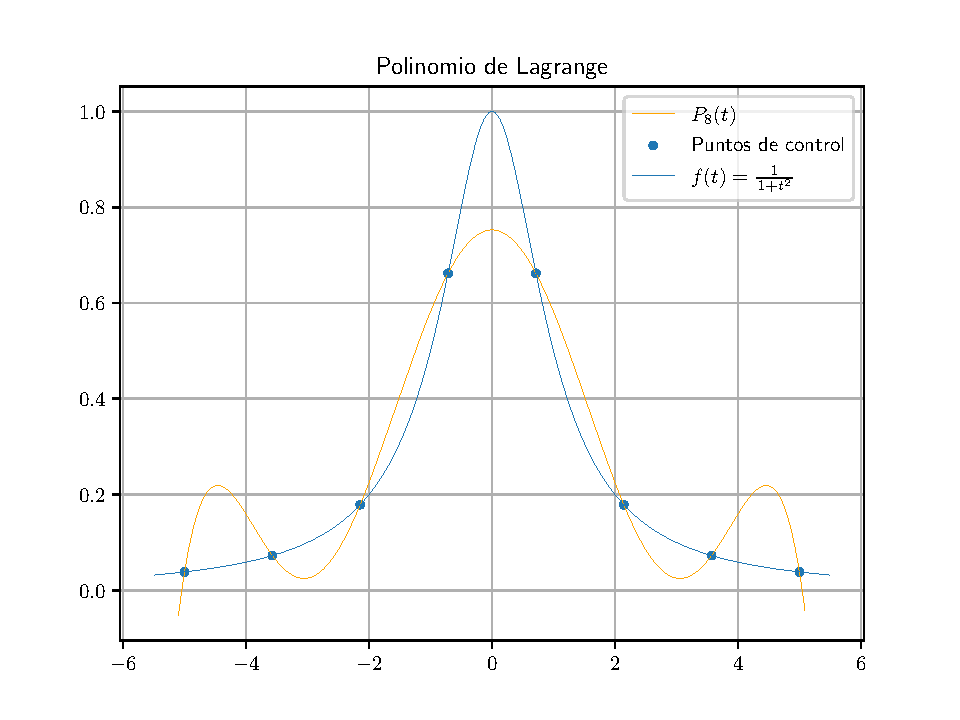
\includegraphics[width=.5\paperwidth]{p12_lagrange8}
        \end{figure}
    \end{solution}
\end{frame}

\begin{frame}
    \begin{solution}
        \begin{equation*}
            P_{9}\left(t\right)=
            -9.099\times 10^{-21}t^{9}+
            5.536\times 10^{-5}t^{8}+
            3.678\times 10^{-19}t^{7}-
            0.002875t^{6}-
            4.312\times 10^{-17}t^{5}+
            0.04917t^{4}+
            6.147\times 10^{-17}t^{3}-
            0.3304t^{2}+
            7.318\times 10^{-17}t+
            0.8615.
        \end{equation*}
        \begin{figure}[ht!]
            \centering
            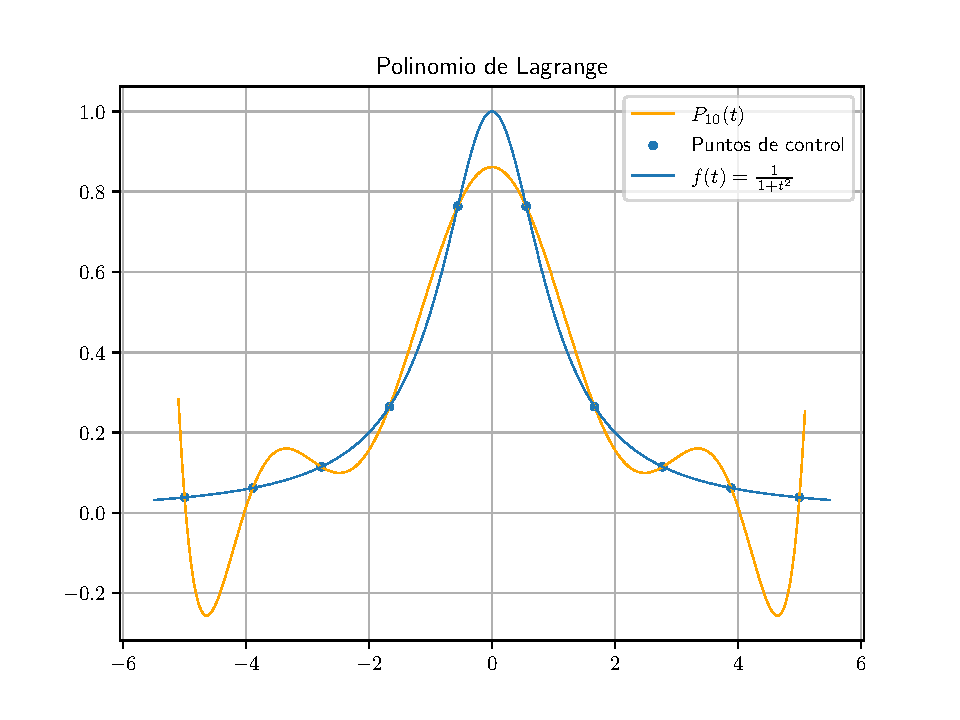
\includegraphics[width=.5\paperwidth]{p12_lagrange10}
        \end{figure}
    \end{solution}
\end{frame}